%\section{Motivation}
\begin{frame}{Motivation}
	\begin{minipage}{\textwidth}
		\centering		
		%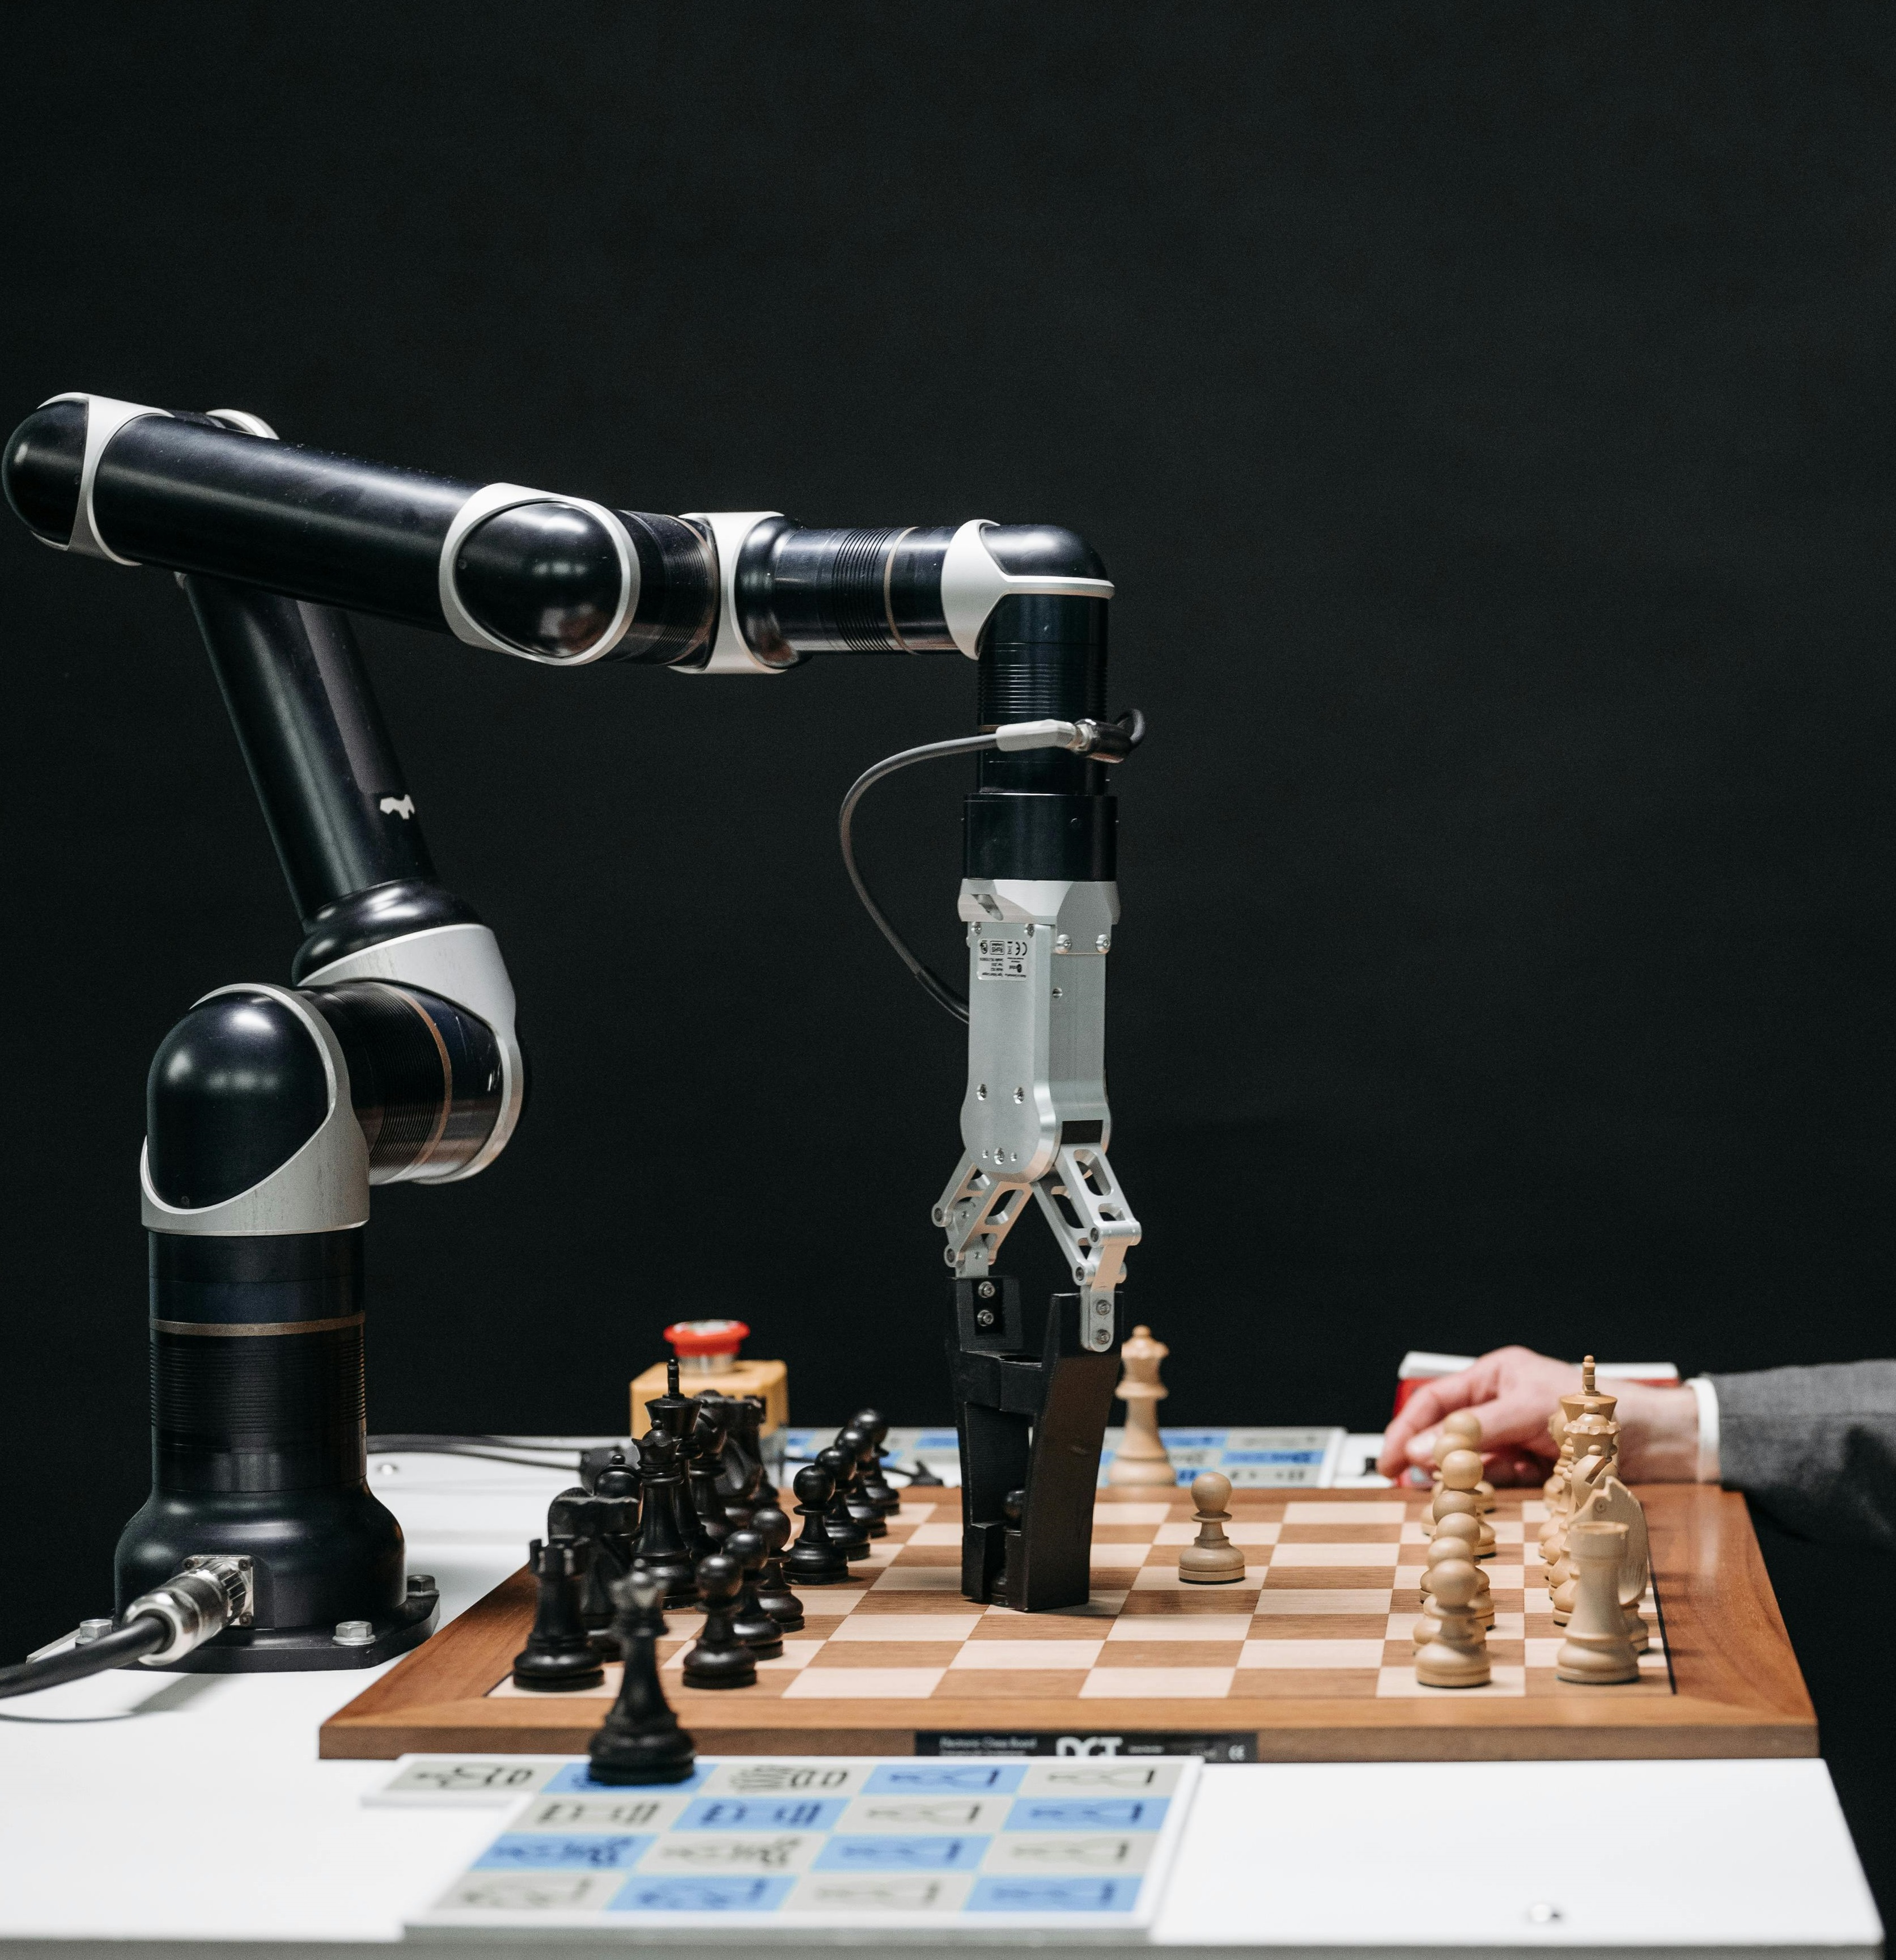
\includegraphics[width=0.2\linewidth]{robotArmGeneric}
		%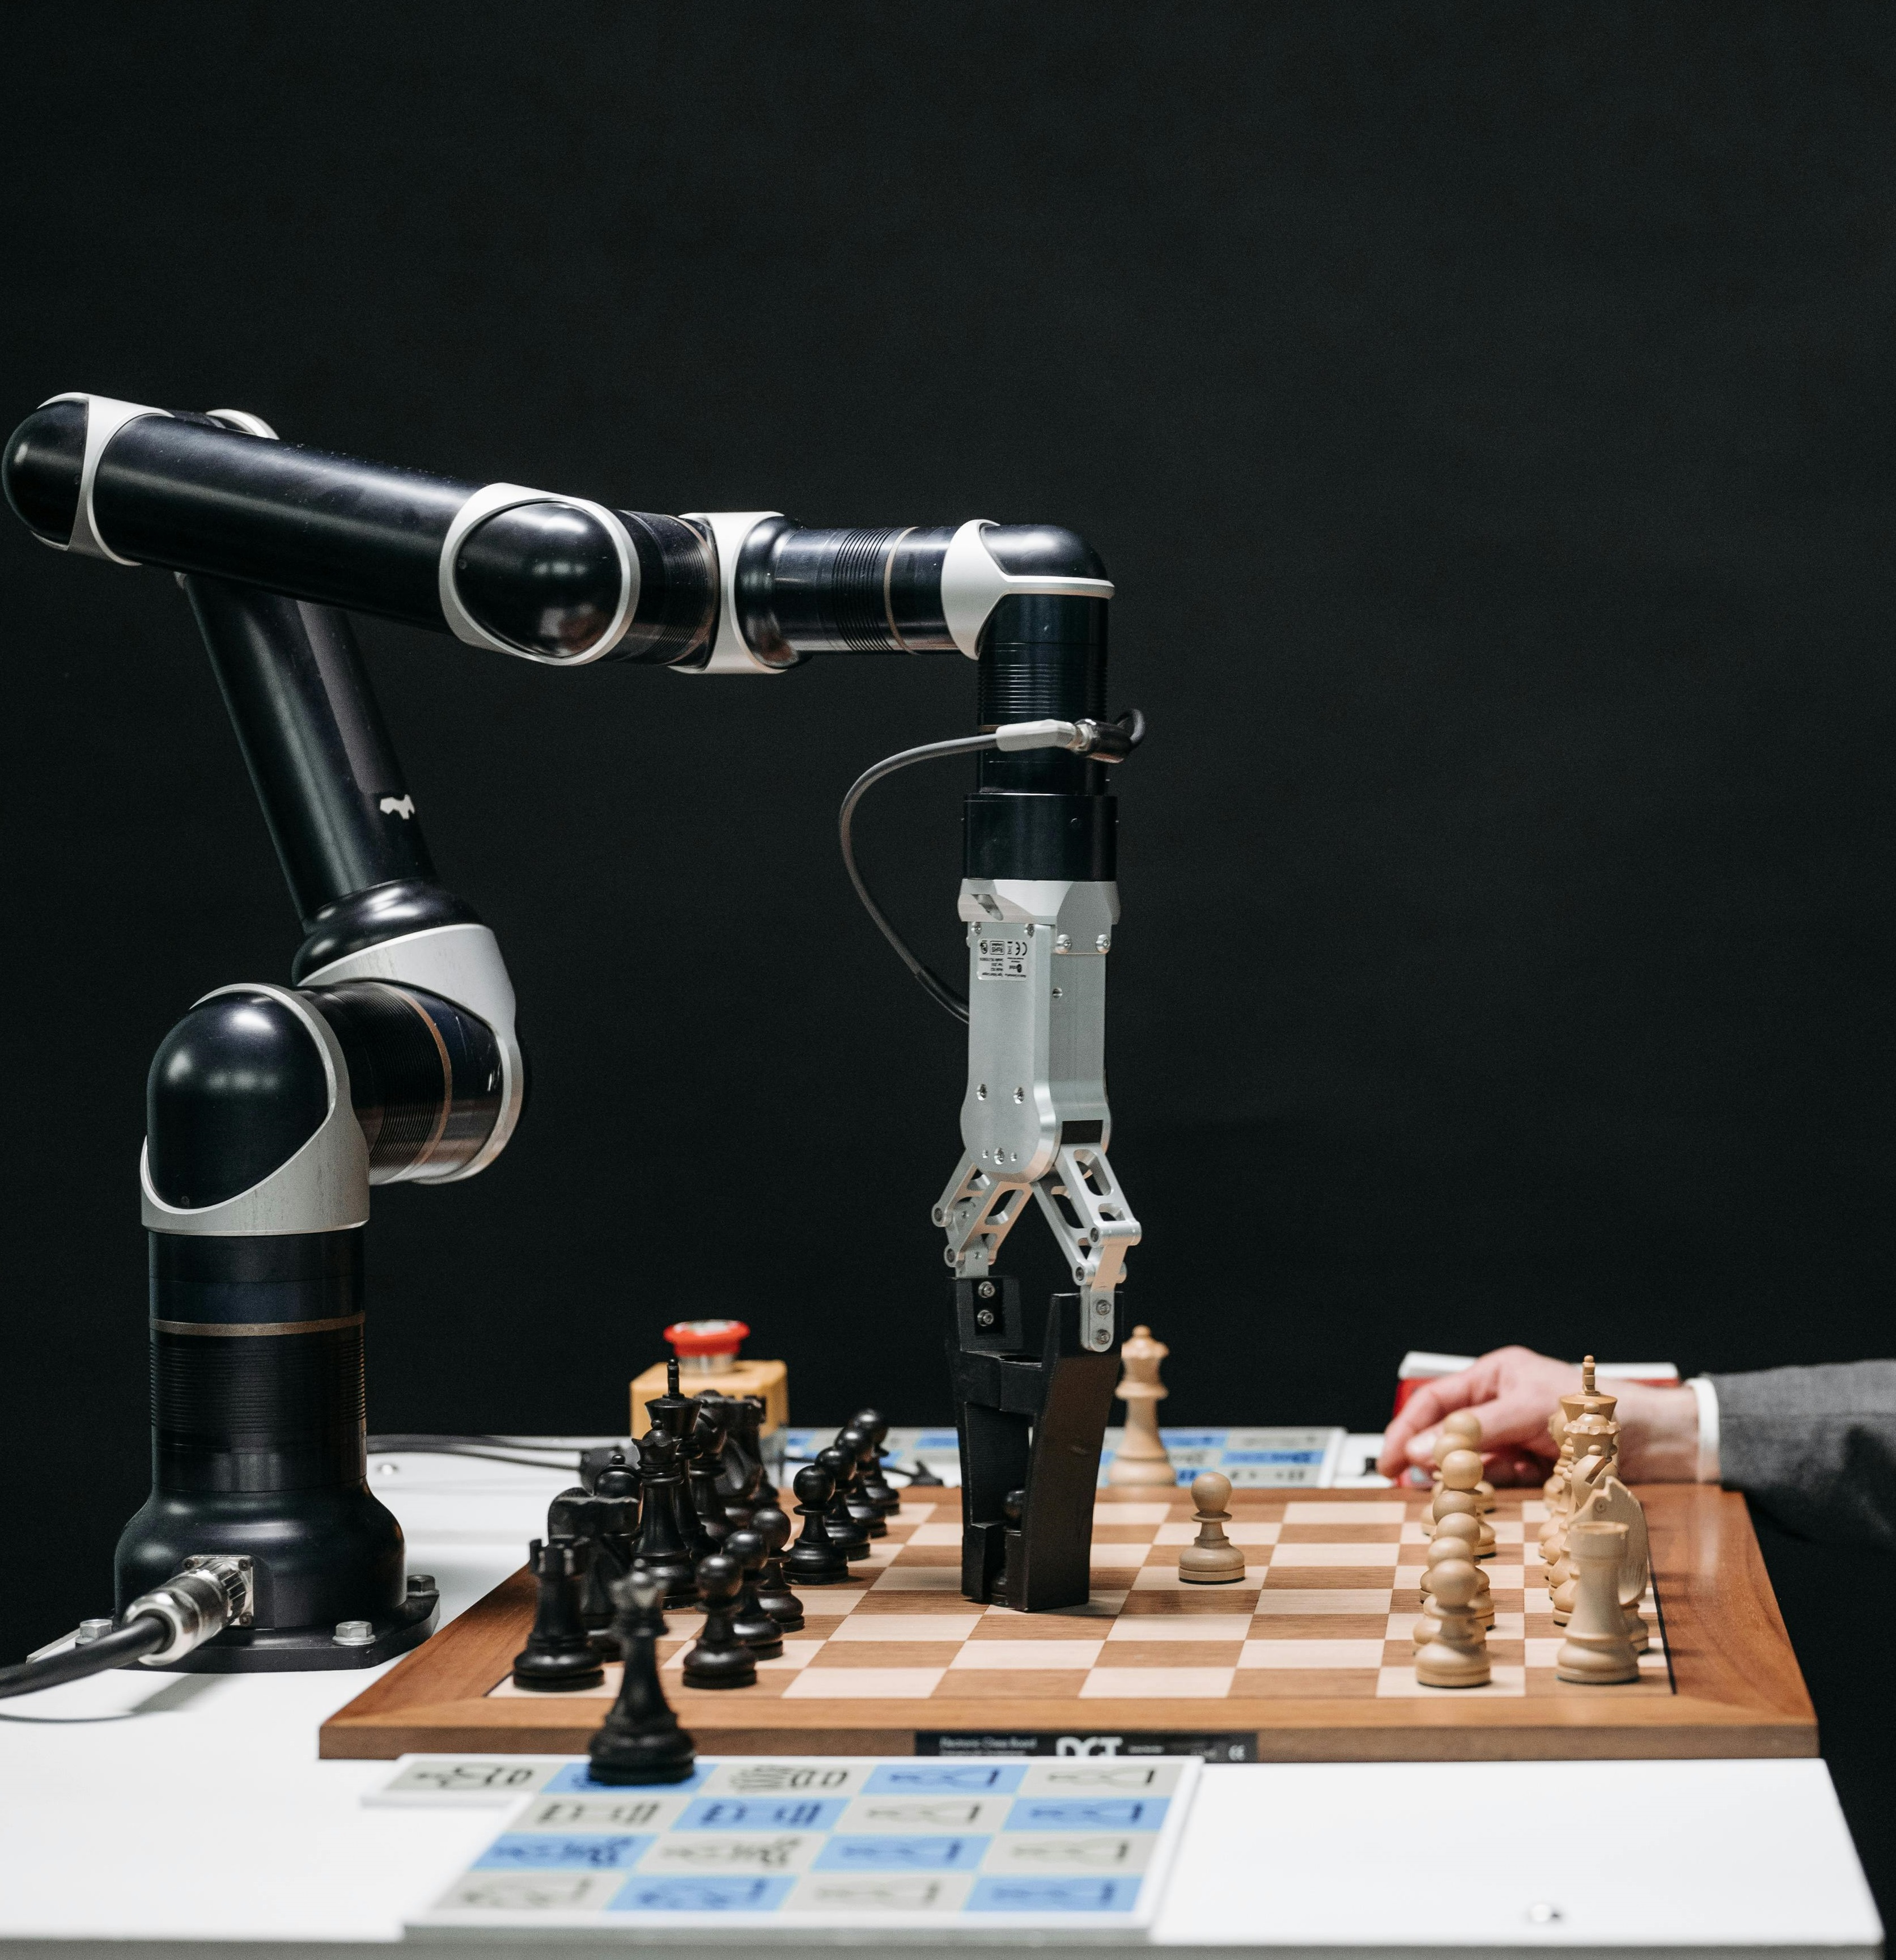
\includegraphics[width=0.5\linewidth]{robotArmGeneric}
		%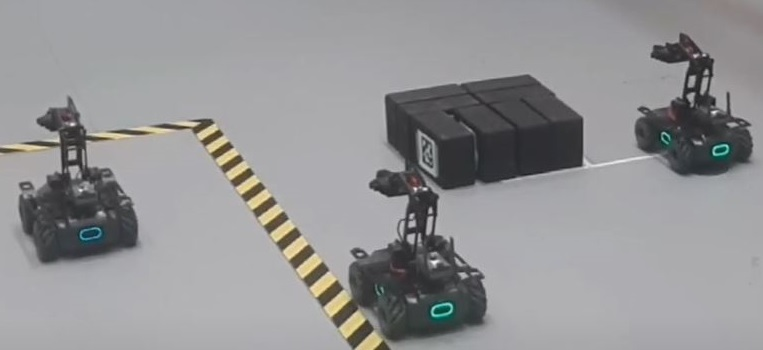
\includegraphics[width=0.2\linewidth]{multiRobotRoboHub}
		%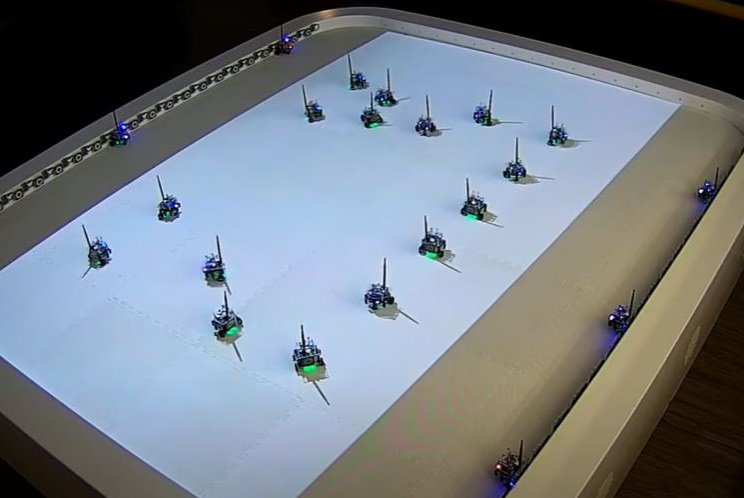
\includegraphics[width=0.2\linewidth]{multiRobotRobotarium}
		%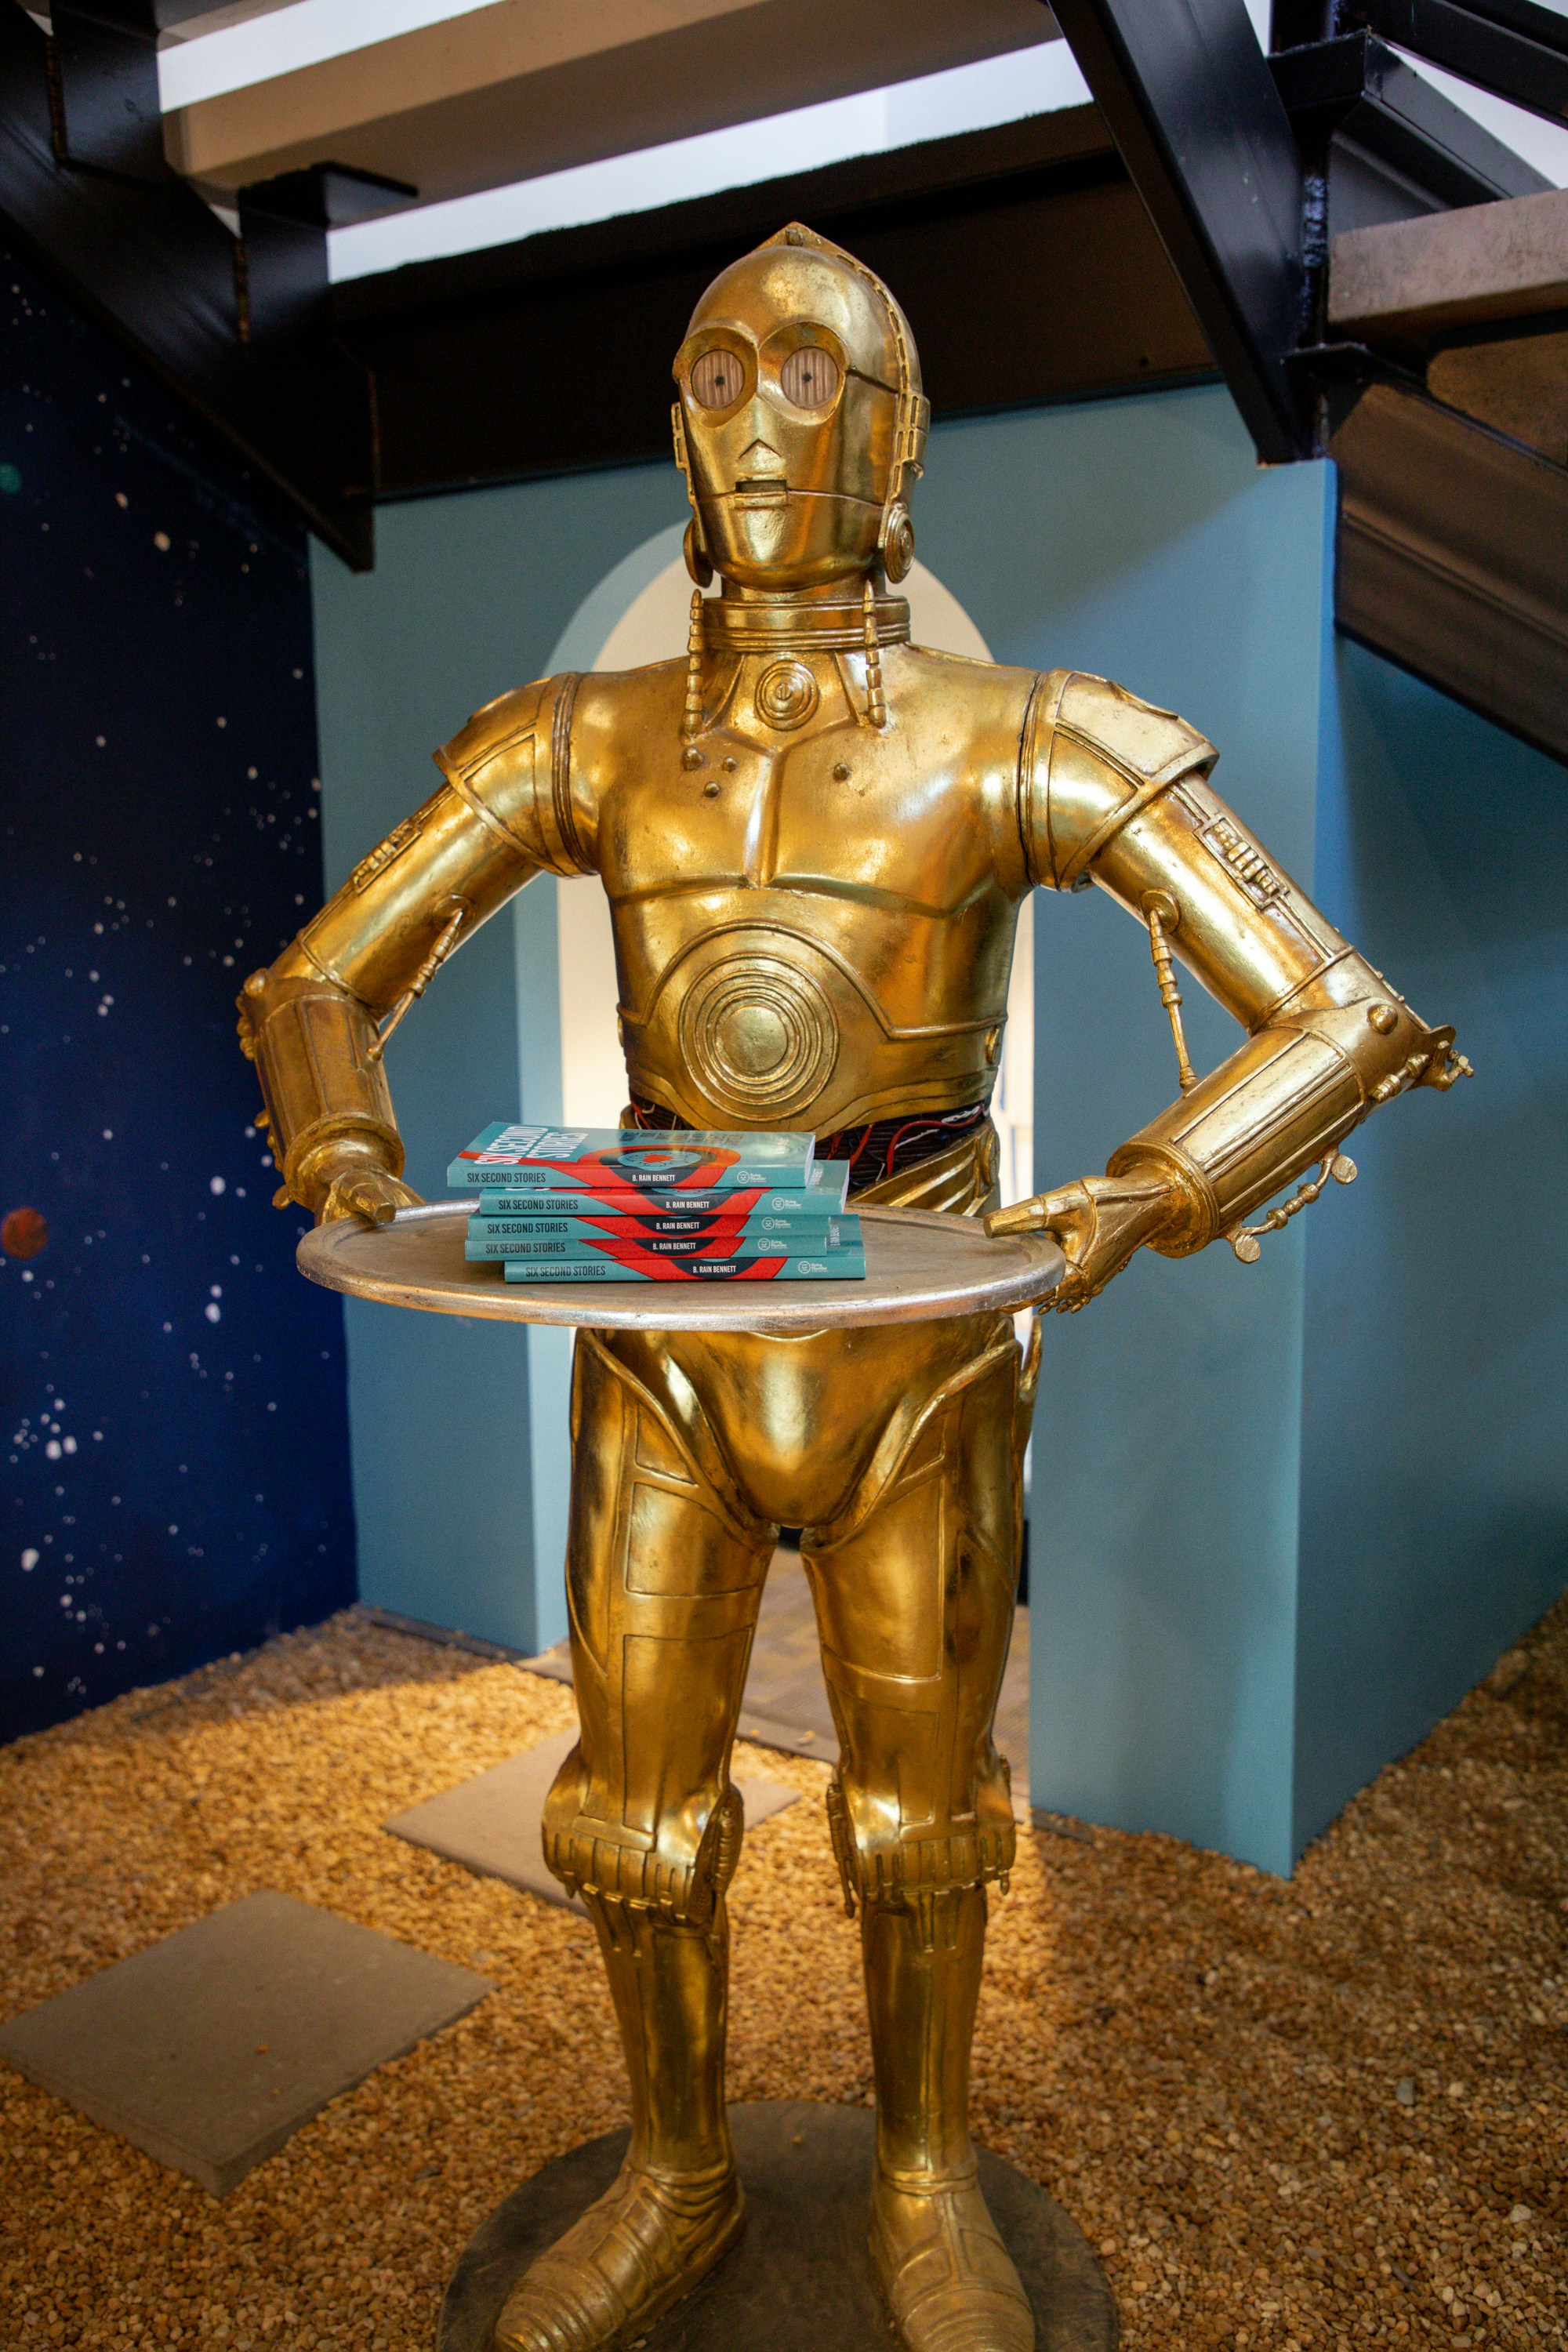
\includegraphics[width=0.2\linewidth]{c3po}
		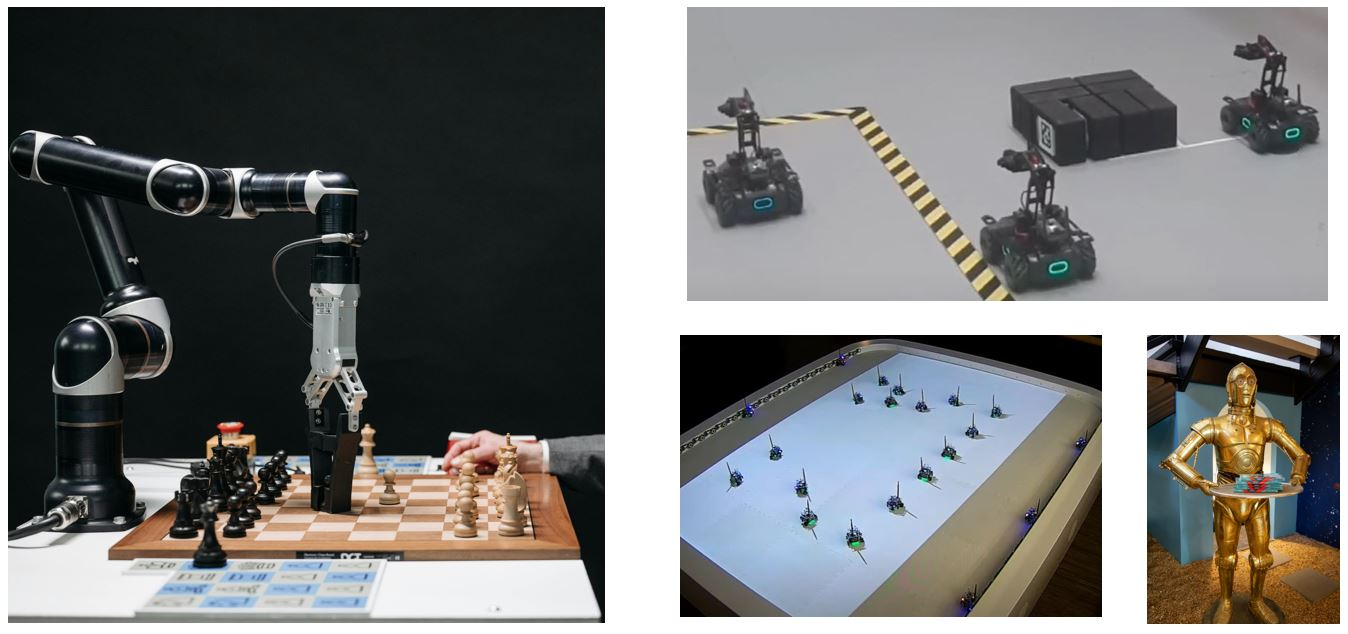
\includegraphics[width=0.85\linewidth]{motivationsCombined}
	\end{minipage}%
	\seprule
	Modern robots are required to do complex tasks and possibly multiple at the same time.
\end{frame}

\begin{frame}
	\begin{itemize}
		\item{Let's use RL to learn several control tasks for a robotic system to execute.}
			\begin{itemize}
				\item{ RL lets us generalize to possibly complex control tasks.}
			\end{itemize}
		\item{Let's combine and execute each of these tasks together.}
			\begin{itemize}
				\item{Preferably in a way that lets us swap out tasks and/or reorder priorities.}
			\end{itemize}
		\item{ { \color{red} How do we know that tasks will not interfere with each other? } }
	\end{itemize}
\end{frame}

\begin{frame}{Assumptions}
	\begin{itemize}
		\item{Assume that our robotic system is control-affine:
	\begin{align*}
		\dot{x} &= f(x) + g(x)u, \,\, x \in \mathbb{R}^n, \,\, u \in \mathbb{R}^p
	\end{align*}}
		\item{Assume that each RL task we learn is encoded with a ``cost-to-go"/value function of the form:
	\begin{align*}
		\tilde{J}_i (x) &\approx \int_t^{\infty} q_i(x(\tau))) + {\lVert u(\tau) \rVert}^2 d \tau, \,\, q_i(x) \ge 0
	\end{align*}}
	\end{itemize}
\end{frame}

\begin{frame}
	Frame without a title
	\begin{itemize}
		\item Frames do not need to have a title...
	\end{itemize}
\end{frame}

\section{Math Expressions}
\begin{frame}{Integrals and Other Expressions}
	\begin{equation}
		\iint_{\partial\Omega}f(x)\diff{x} \in \complexes
	\end{equation}
	\begin{align}
		E &= mc^2\\
		F &= ma
	\end{align}

	\seprule
	
	\begin{tabular}{rl}
		$m$ & Mass\\
		$c$ & Speed of light
	\end{tabular}
\end{frame}
\begin{frame}{Theorems, Lemmas, ...}
	\begin{thm}
		The following statement is correct
		\begin{equation}
			\frac{\partial f(\vec{x})}{\partial x_i} = \sum_{l=1}^{L}\cos\left(l\frac{2\pi}{L} + 0\right)
		\end{equation}
	\end{thm}
\end{frame}

\section{Elements}

\begin{frame}[fragile]{Typography}
	\begin{verbatim}The theme provides sensible defaults to
		\emph{emphasize} text, \alert{accent} parts
		or show \textbf{bold} results.\end{verbatim}
	
	\begin{center}becomes\end{center}
	
	The theme provides sensible defaults to \emph{emphasize} text,
	\alert{accent} parts or show \textbf{bold} results.
\end{frame}

\begin{frame}{Font feature test}
	\begin{itemize}
		\item Regular
		\item \textit{Italic}
		\item \textsc{Small Caps}
		\item \textbf{Bold}
		\item \textbf{\textit{Bold Italic}}
		\item \textbf{\textsc{Bold Small Caps}}
		\item \texttt{Monospace}
		\item \texttt{\textit{Monospace Italic}}
		\item \texttt{\textbf{Monospace Bold}}
		\item \texttt{\textbf{\textit{Monospace Bold Italic}}}
	\end{itemize}
\end{frame}

\begin{frame}{Lists}
	\begin{columns}[T,onlytextwidth]
		\column{0.33\textwidth}
		Items
		\begin{itemize}
			\item Milk \item Eggs \item Potatoes
		\end{itemize}
		
		\column{0.33\textwidth}
		Enumerations
		\begin{enumerate}
			\item First, \item Second and \item Last.
		\end{enumerate}
		
		\column{0.33\textwidth}
		Descriptions
		\begin{description}
			\item[PowerPoint] Meeh. \item[Beamer] Yeeeha.
		\end{description}
	\end{columns}
\end{frame}
\begin{frame}{Tables}
	\begin{table}
		\caption{Largest cities in the world (source: Wikipedia)}
		\begin{tabular}{@{} lr @{}}
			\toprule
			City & Population\\
			\midrule
			Mexico City & 20,116,842\\
			Shanghai & 19,210,000\\
			Peking & 15,796,450\\
			Istanbul & 14,160,467\\
			\bottomrule
		\end{tabular}
	\end{table}
\end{frame}
\begin{frame}{Blocks}
	Three different block environments are pre-defined and may be styled with an
	optional background color.
	
	\begin{columns}[T,onlytextwidth]
		\column{0.45\textwidth}
		\begin{block}{Default}
			Block content.
		\end{block}
		
		\begin{alertblock}{Alert}
			Block content.
		\end{alertblock}
		
		\begin{exampleblock}{Example}
			Block content.
		\end{exampleblock}
		
		\column{0.45\textwidth}
		
		\metroset{block=fill}
		
		\begin{block}{Default}
			Block content.
		\end{block}
		
		\begin{alertblock}{Alert}
			Block content.
		\end{alertblock}
		
		\begin{exampleblock}{Example}
			Block content.
		\end{exampleblock}
		
	\end{columns}
\end{frame}
\begin{frame}{Line plots}
	\begin{figure}
		\begin{tikzpicture}
			\begin{axis}[
				betterplot,
				width=0.9\textwidth,
				height=6cm,
				]
				
				\addplot {sin(deg(x))};
				\addplot+[samples=100] {sin(deg(2*x))};
				
			\end{axis}
		\end{tikzpicture}
	\end{figure}
\end{frame}

\begin{frame}[standout,plain]
	Standout Frame!
\end{frame}


\appendix
\begin{frame}[fragile]{Backup slides}
	Sometimes, it is useful to add slides at the end of your presentation to
	refer to during audience questions.
	
	The best way to do this is to include the \verb|appendixnumberbeamer|
	package in your preamble and call \verb|\appendix| before your backup slides.
	
	The theme will automatically turn off slide numbering and progress bars for
	slides in the appendix.
\end{frame}
